\documentclass[12pt, letterpaper, twoside]{article}
    \usepackage[utf8]{inputenc}
    \usepackage{graphicx}
    \usepackage{fullpage}
    \usepackage{pgfplotstable}
    \usepackage{amsmath, amssymb}
    
\title{Homework 3 Report}
\date{November 15, 2018}
\author{Sean Kane}

\begin{document}
\maketitle
% \centerline{\textbf{Homework 3 Report}}
% \centerline{\textbf{Sean Kane}}
\section{Problem 1}
MNIST Neural Network

\subsection{System Description}
Description of all choices made - num of hidden neurons, learning rate, momentum, output thresholds, 
rules for choosing initial weights, criterion for deciding when to stop training, etc

This neural network is built with 784 input layers - each corresponding to one pixel of a 28 x 28 
image - 150 hidden neurons, and ten output neurons. Each of the ten output neurons corresponded to an
identified number. For example, if the output of the zeroth neuron was a one, this would predict a 
zero, a one at the first neuron meant a prediction of one. A learning rate of 0.01 and an alpha value 
of 0.5 was used for the implementation of momentum. 

During training the output threshold was determined by which neuron had the highest output value of 
over 0.75. If there was not a neuron over 0.75, the outputwas null and the system was trained as if 
it was incorrect. During testing, the predicted neuron was the neuron with the highest value, regardless
of whether it was over 0.75. 

Training of the neural network occurred until one of two conditions was met. The first condition was a 
maximum number of epochs set at 800. This number was chosen because I wanted the machine to see each 
test point an average of ten times, and with a mini batch size of 50 and a test sample size of 4000, 
the epoch on average would be 800. The second condition, which occassionally would cause training to end
before the max epochs, was if the percent change in loss dropped below .01 percent. Percent change was 
measured as:
% \begin{equation}
        
    % $Percent Change$ = \frac{$Loss_{N-1}-Loss_{N}$}{$Loss_{N-1}$}
    % (LossEpochN-1 - LossEpochN) / (LossEpochN-1) * 100
% \end{equation}
\[
    PercentChange = \frac{  Loss_{N-1} - Loss_{N}  }{ Loss_{N-1}   }%k!(n-k)!}
\]


\subsection{Results}
Performance of final network on training and test set using confusion matrix.
Plot time series of error during training saved every tenth epoch
Testing accuracy: 0.8461 after 297 epochs.

\subsection{Confusion Matrix}

\pgfplotstabletypeset{confusionmatrix.csv} %[dec sep align, fixed zerofill, precision=0, col sep=space]{confusionmatrix.csv}
\end{table}

\subsection{Error Rate Graph}
\begin{figure}
    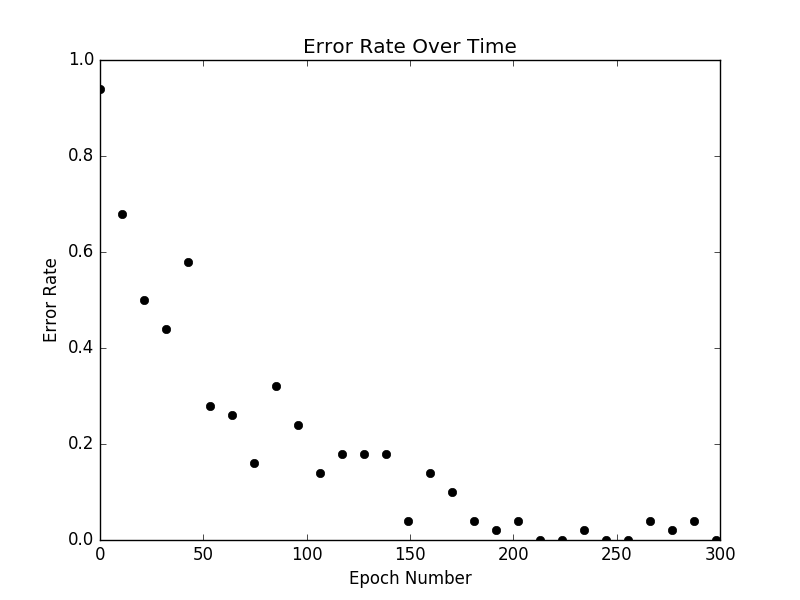
\includegraphics[scale=0.5]{NNErrorRate}
    % \caption{Error Rate}
\end{figure}

\subsection{Analysis of Results}
Describe, discuss, and interpret results you got, and why you think they as as they are.

\section{Problem 2}
Autoencoder

\subsection{System Description}
Description of learning rate, momentum, initial weights, when to stop training.

\subsection{Results}
Performance of final network on the training set adn test set. Two values which 
should be plotted as two bars side by side. Plot same error in the same way, separated
by each digit - two bars for 0, two for 1, etc. Plot time series of the overall
training error during training using the data saved at every tenth epoch.

\subsection{Features}
Plot images for a large number of features, just like data shown in first100.jpg

\subsection{Analysis of Results}
Describe, discuss, and interpret results you got and why you think they are. Comment
on features you found, and what they suggest. Comment on which digits turned out to be 
easiest to reconstruct and which ones more difficult, and why you think that happened.


\end{document}